\begin{frame}[c]
	\myframetitle{Task 3.1 }{Erste Verwendung der libsvm}
\begin{itemize}
  \fatitem Der Erste Test wurde mit 1600 Features durchgeführt
  \begin{itemize}
    \item Das Training dauerte 4193ms
    \item Die Klassifikation dauerte 3266ms
    \item Accuracy = 78.14% (411/526) (classification)
    \item Die Gesamtlaufzeit betrug 7460ms
  \end{itemize}
\end{itemize}
\end{frame}



\begin{frame}[c]
	\myframetitle{Task 3.2 }{Genauigkeit in Abhängigkeit der Features}
%\usepackage{graphics} is needed for \includegraphics
\begin{figure}[htp]
\begin{center}
  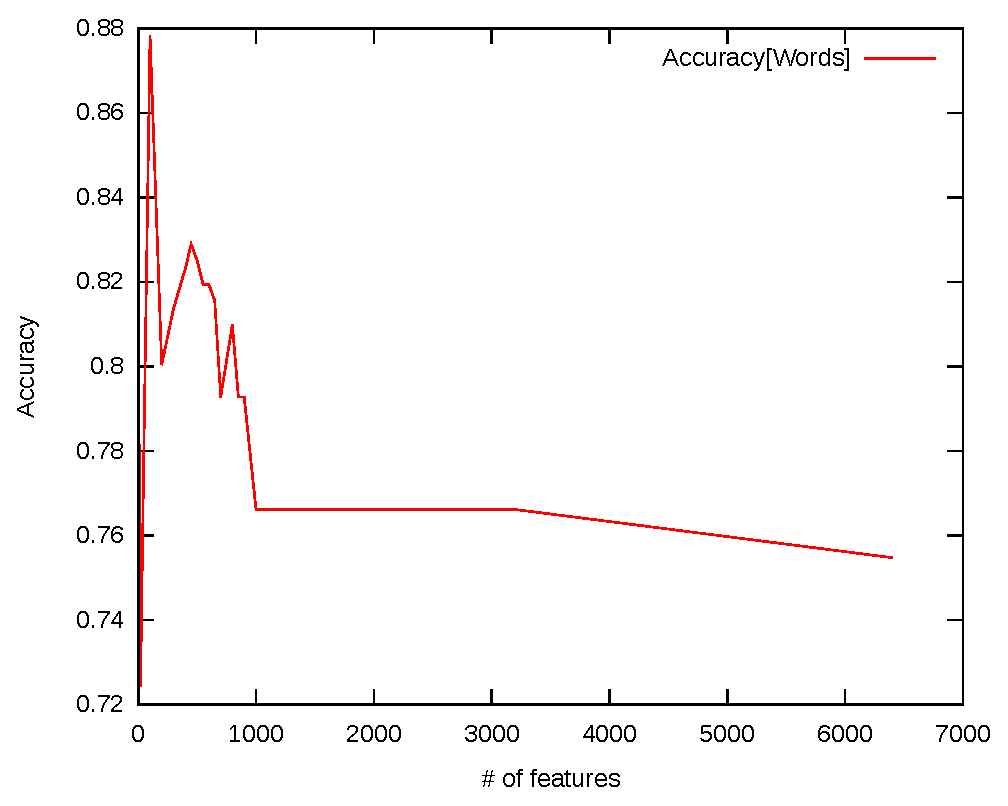
\includegraphics[width=0.5\textwidth]{graphics/accuracy_tokens}
  \caption[labelInTOC]{Genauigkeit in Abhängigkeit der Features bei der
  Verwendung aller Worte}
  \label{fig:tokenAccuracy}
\end{center}
\end{figure}
\end{frame}
	
	\begin{frame}[c]
	\myframetitle{Task 3.2 }{Performanz in Abhängigkeit der Features}
%\usepackage{graphics} is needed for \includegraphics
\begin{figure}[htp]
\begin{center}
  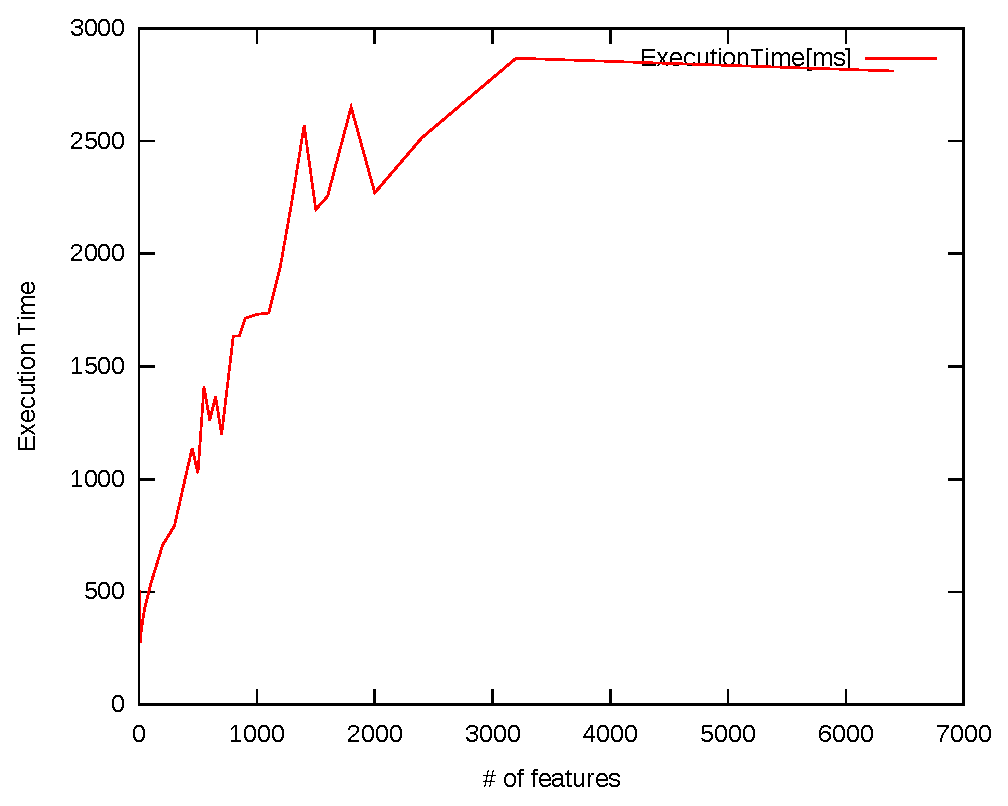
\includegraphics[width=0.5\textwidth]{graphics/exec_tokens}
  \caption[labelInTOC]{Zeitdauer(ms) in Abhängigkeit der Features bei der
  Verwendung aller Worte}
  \label{fig:tokenAccuracy}
\end{center}
\end{figure}
\end{frame}
	
	
	\begin{frame}[c]
	\myframetitle{Task 3.3 }{Vergleich der Präzision zwischen Stem- und
	Stopwortentfernung}
%\usepackage{graphics} is needed for \includegraphics
\begin{figure}[htp]
\begin{center}
  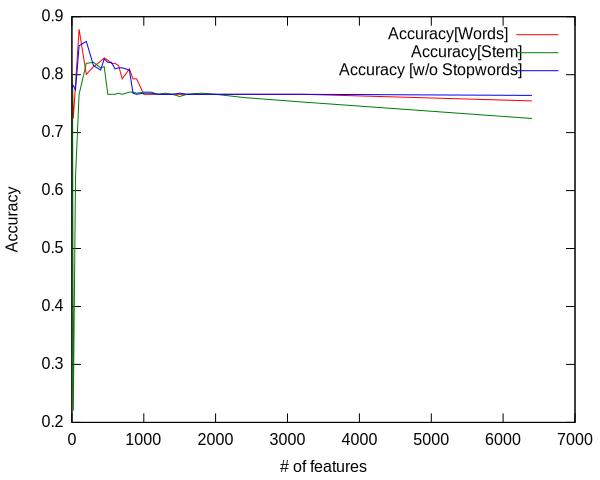
\includegraphics[width=0.5\textwidth]{graphics/accuracy_comparison}
  \caption[labelInTOC]{Genauigkeit in Abhängigkeit der Features im Vergleich}
  \label{fig:tokenAccuracy}
\end{center}
\end{figure}
\end{frame}

\begin{frame}[c]
	\myframetitle{Task 3.3 }{Vergleich der Dauer zwischen Stem- und
	Stopwortentfernung}
%\usepackage{graphics} is needed for \includegraphics
\begin{figure}[htp]
\begin{center}
  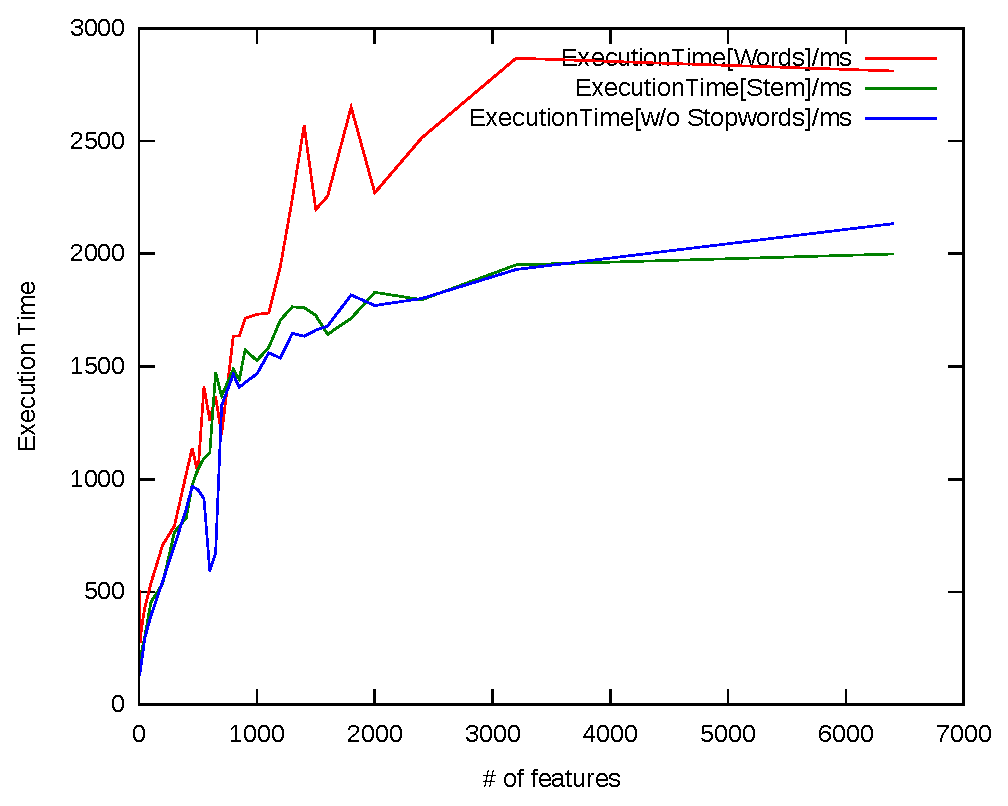
\includegraphics[width=0.5\textwidth]{graphics/exec_comparison}
  \caption[labelInTOC]{Zeitdauer(ms) in Abhängigkeit der Features im
  Vergleich}
  \label{fig:tokenAccuracy}
\end{center}
\end{figure}
\end{frame}

\begin{frame}[c]
	\myframetitle{Task 3.3 }{Interpretation der Ergebnisse}
%\usepackage{graphics} is needed for \includegraphics
\begin{itemize}
  \item{Die Präzision wird maximal bei etwa 250\ldots300 Features}
  \item{Für unendlich viele Features geht die Präzision gegen das Verhältnis
  zwischen Course- und Noncourse-Websites}
  \begin{itemize}
  \fatitem{ $\rightarrow$ Es dürfen nicht zu viele Features verwendet werden}
  \end{itemize}
  \item Das Entfernen der Stopworte verringert die Ausführungszeit der
  Klassifikation deutlich.
  \begin{itemize}
  \item Stopworte kommen in allen Dokumenten oft vor
  \item Durch die Feature-Selektion werden die Stoppworte daher häufig als
  Features gewertet
  \item Die Verwendung von Stopworten als Features verringert den Abstand
  zwsichen den Klassen in der Hyperebene 
  \item Der SVM-Algorithmus konvergiert langsamer
\end{itemize}
\end{itemize}
\end{frame}

\begin{frame}[c]
	\myframetitle{Task 3.3 }{Interpretation der Ergebnisse2}
%\usepackage{graphics} is needed for \includegraphics
\begin{itemize}
  \item Stoppwortentfernung beeinflusst die Zeitdauer der Vorverarbeitung kaum
  \item Stemming beeinflusst die Zeitdauer der Vorverarbeitung ebenfalls kaum
  \fatitem{In dieser Messung hat aber das Stemming die Präzision verringert}
  \begin{itemize}
  \item Daher sollte bei diesem Klassifikationsproblem auf Stemming verzichtet
  werden.
\end{itemize}
  \item Die Stoppwortentfernung als Vorverarbeitung ist allerdings sinnvoll.
\end{itemize}
\end{frame}

\begin{frame}
  \myframetitle{Task 3.3}{Präzision ist nicht alles}
\begin{itemize}
  \item Bei der Verwendung eines Klassifikationsverfahrens muss immer ein
  Tradeoff zwischen Kosten und Leistung gefunden werden.
  \fatitem{Wenn das Verfahren mit der höchste Präzision zu teuer ist, muss ein
  kostengünstigeres Verfahren gefunden werden.}
  \item Daher wird Lemmatisierung nicht verwendet, um den Wortstamm präzise zu
  bestimmen.
  \item Stattdessen kommt Stemming zum Einsatz, auch wenn die Ergebnisse des
  Stems möglicherweise linguistisch betrachtet falsch sind.
\end{itemize}
\end{frame}
	
\begin{frame}
  \myframetitle{Task 3.4}{Vergleich verschiedener Kernel}
  \begin{itemize}
  \item Bei 50 Features:
  \item Linear: 
  \begin{itemize}
  \item Präzision(Test) 84.60\%,
  \item Präzision(Training)  96.76\%
  \item Training: 640ms, Klassifikation: 112ms
\end{itemize}
  \item Polynomial:
  \begin{itemize}
  \item Präzision(Test) 78.13\%,
  \item Präzision(Training)  78.09\%
  \item Training: 544ms, Klassifikation:
  96ms
\end{itemize}
  \item RBF: 
  \begin{itemize}
  \item Präzision(Test) 78.40\%,
  \item Präzision(Training)  78.28\%
  \item Training: 640ms,  Klassifikation: 112ms
\end{itemize}
     \fatitem{$\rightarrow$Bei wenigen Features trennt ein linearer Kernel am
     besten}
\end{itemize}
\end{frame}

\begin{frame}
  \myframetitle{Task 3.5}{Optimierung von c, g, o.Ä}
  \begin{itemize}
  \item Bei 50 Features:
  \item Linear: 
  \begin{itemize}
  \item Präzision(Test) 84.60\%,
  \item Präzision(Training)  96.76\%
  \item Training: 640ms, Klassifikation: 112ms
\end{itemize}
  \item Polynomial:
  \begin{itemize}
  \item Präzision(Test) 78.13\%,
  \item Präzision(Training)  78.09\%
  \item Training: 544ms, Klassifikation:
  96ms
\end{itemize}
  \item RBF: 
  \begin{itemize}
  \item Präzision(Test) 78.40\%,
  \item Präzision(Training)  78.28\%
  \item Training: 640ms,  Klassifikation: 112ms
\end{itemize}
     \fatitem{$\rightarrow$Bei wenigen Features trennt ein linearer Kernel am
     besten}
\end{itemize}
\end{frame}

	
	
	